\documentclass[times, twoside, watermark]{zHenriquesLab-StyleBioRxiv}
\usepackage{preamble}

% Please give the surname of the lead author for the running footer
\leadauthor{Raunak Redkar} 

\begin{document}

\title{Rapid Sequence Similarity Detection with Bloom Filters and Locality-Sensitive Hashing}
\shorttitle{Sequence Similarity Detection}

% Use letters for affiliations, numbers to show equal authorship (if applicable) and to indicate the corresponding author
\author[1, 2 ]{Raunak Redkar }
\author[1, 2, 3 ]{Cynthia Wang } 
\author[2, 4 ]{Mark Chernyshev }

\affil[1]{Summer Research School in Computational Biology and Bioinformatics, Karolinska Institutet.}

\affil[2]{Department of Microbiology, Tumor and Cell Biology, Karolinska Institutet.}

\affil[3]{Lab partner}

\affil[4]{Project Supervisor}

\maketitle

%TC:break Abstract
%the command above serves to have a word count for the abstract
\begin{abstract}
Several exact and approximate similarity detection algorithms run in $O(n^2)$ or $O(n\log n)$ time. In this paper, we explore linear time probabilistic methods for identifying index hopping that can occur during a gene sequencing run and for clustering antibody clonal lineages that arise during somatic hypermutation. For index hopping, finding exact sequence matches between datasets are implented using Bloom Filters, a memory efficient data structure. For clustering clonal lineages, we opt for the method of Locality-Sensitive Hashing (LSH) to collide similar sequences into the same hash bucket with a high probability. Bloom Filters are found to detect sequence contamination between datasets successfully while maintaining a low memory usage and runtime. Furthermore, we demonstrate that Locality-Sensitive Hashing managed to cluster similar sequences to some degree. However, the pairwise Jaccard Index show that the LSH clusters do not resemble the clusters generated by single-linkage clustering, hence further testing and analysis is required to determine the method's viability. 
\end{abstract}
%TC:break main
%the command above serves to have a word count for the abstract

\begin{keywords}
Index Hopping | Bloom Filters | Clonal Lineages | Locality-Sensitive Hashing 
\end{keywords}

\begin{corrauthor}
raunak.redkar\at gmail.com
\end{corrauthor}

\section*{Introduction}

\section*{Antibodies}
A key aspect of the immune system is diversity, as the pathogens encountered by living organism can be highly varied. By consequence of this, living organisms have evolved to have immune mechanisms that can deal with high diversity. One of these mechanisms is the productions of antibodies, diverse proteins that protect the host from pathogens by binding to them in order to signal the immune system or prevent the pathogen's functioning.

\subsection*{VDJ Recombination}
VDJ-recombination is a part of somatic recombination, which is a type of gene rearrangement that the adaptive immune system performs in developing lymphocytes. During VDJ-recombination, V, D and J genes are randomly combined by first splicing introns and then recombining the VDJ exons to make a naive antibody coding sequence. These VDJ gene segments are specifically responsible for the variable regions on the antibody that bind to the antigen - heavy and light chains. The complementarity-determining region 3 (CDR3) coding nucleotide region lies on the VDJ region, fully covering the D exon. It is the most variable complementarity-determining region (CDR), and thus is crucial for generating diversity in the host's antigen specificity repertoire. \cite{vdjRecombination} 

% wtf is cdr3

\subsection*{Somatic Hypermutation}
Somatic hypermutation (SHM) is a process where point mutations happen in the variable gene regions in the antibody; the heavy and light chains. B-cells that have high affinity for binding to antigen receptors send out signals and proliferate and undergo somatic hypermutation. This results in more activated B-cells that can potentially differentiate into antibody secreting plasma cells. SHM occurs more in the variable regions of the antibodies that affect antigen binding. The key aspect of SHM is to generate diversity in terms of antigen-antibody interaction in a hillclimbing process to increase the chance of developing the best antibodies. \cite{vdjRecombination} 

\section*{Index hopping}
Multiplex sequencing is when multiple samples are combined in a single gene sequencing run. This is done to increase the speed and magnitude of sequencing in order to save time and money. Prior to sequencing, the DNA fragments in a sample are marked with i7 and i5 adapters which are unique to that sample. The DNA fragments from all samples are pooled and then sequenced. The result is a mix of sequencing reads from different samples/donors/libraries. During this process, spill over or leakage can occur from one sample to another, which can result in the incorrect adaptors being assigned to a sequence - \textit{index hopping}. The popular way to deal with this has been to do pairwise comparisons between the libraries, to see if sequences exist in other libraries as well. Since we are working with VDJ sequences, which are highly diverse, identical sequences in two libraries are highly likely to be a sign of leakage. We opt for a Bloom Filter based set inclusion check in order to reduce the memory for checking leakage. This part of the project is exact matching between sequences. \cite{indexHopping}

\subsection*{Sequence representation}

\subsubsection{One-hot encoding}
In statistics and machine learning, a one-hot is a group of bits where one bit is turned on while the others are turned off. This works very intuitively with biological gene sequences. We represent each nucleotide with 4 bits: where the 1st, 2nd, 3rd, or 4th is turned on if the nucleotide is A, C, G, or T respectively. For example, the one-hot encoding for "ACGTA" is $10000100001000011000$. By their nature, one-hot encoded sequences preserve the order of the nucleotides well.  
\subsubsection{K-mer Vectors}
A k-mer is a substring in a biological nucleotide sequence which is of length $k$. As there are 4 possible nucleotides, there are $4^{k}$ possible k-mers. A sequence can then be represented by a \textit{k-mer vector} of length $4^{k}$ which contains the k-mer counts of all k-mers in the sequence. The advantage of k-mer vectors is that, unlike one-hot encoding, they have a fixed length which means that gene sequences of any length can be reduced to a universal format that can be processed in the same way every time.

\subsection*{Bloom Filters}
A bloom filter is a memory efficient data structure for querying inclusion in a set. It is a bitarray, where the bits turned on represent the elements in the set. When inserting an element, $k$ hash functions each hash the element into a specific index, which is turned on in the bitarray. The trade-off for space-efficiency is that data structure is probabilistic - false positives are possible. The false positive rate is a function of the number of hash functions $k$ and the number of bits $m$ in the bitarray. \cite{BloomFilters}

\section*{Antibody lineages}

VDJ recombination and somatic hypermutation is a type of evolutionary hillclimbing process that attempts to produce the best antibody suited for the pathogen. In this process, clonal lineages can form which are sets of B-cells which descend from one another through mutations occurring during somatic hypermutation. These clonal lineages tend to have sequences of the same length, as insertions and deletions are not common. Data clustering algorithms attempt to cluster these clonal lineages. 


\subsection*{Single-linkage clustering}
Single-linkage clustering is a type of hierarchical clustering. Initially, every element is its own cluster. Then at every step, the two pairs of points with the minumum distance which are not yet in the same cluster are grouped together until all elements are in the same cluster. This process of clustering makes a tree which can be represented by a dendrogram. Single-linkage clustering of CDR3 sequences is the standard method for grouping antibody lineages. \cite{singleLinkage} 

% figure of a dendrogram 
\begin{figure}[!h]
    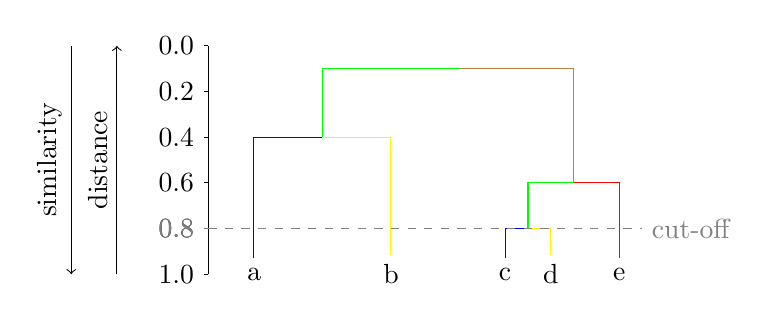
\begin{tikzpicture}[sloped, scale = 0.58]
        \node (a) at (-6,0) {a};
        \node (b) at (-3,0) {b};
        \node (c) at (-0.5,0) {c};
        \node (d) at (0.5,0) {d};
        \node (e) at (2,0) {e};
        \node (ab) at (-4.5,3) {};
        \node (cd) at (0,1) {};
        \node (cde) at (1,2) {};
        \node (all) at (-1.5,4.5) {};
        
        \draw[color = blue]  (a) |- (ab.center);
        \draw[color = yellow]  (b) |- (ab.center);
        \draw[color = blue]  (c) |- (cd.center);
        \draw[color = yellow]  (d) |- (cd.center);
        \draw[color = red]  (e) |- (cde.center);
        \draw[color = green]  (cd.center) |- (cde.center);
        \draw[color = green]  (ab.center) |- (all.center);
        \draw[color = brown]  (cde.center) |- (all.center);
        
        \draw[<-] (-10,0) -- node[above]{similarity} (-10,5);    
        \draw[->] (-9,0) -- node[above]{distance} (-9,5);
        
        \draw (-7,0) -- (-7,5);
        
        \foreach \y in {0,1,2,3,4,5}                     
        \draw[shift={(0,\y)},color=black] (-7,0) -- (-7.1,0);
        
        \node[left] at (-7.1,0) {$1.0$} ;
        \node[left] at (-7.1,1) {$0.8$} ;
        \node[left] at (-7.1,2) {$0.6$} ;
        \node[left] at (-7.1,3) {$0.4$} ;
        \node[left] at (-7.1,4) {$0.2$} ;
        \node[left] at (-7.1,5) {$0.0$} ;
        
        \draw[dashed,color=gray] (-7,1) -- node[at end, right]{cut-off} (2.5,1);
        \draw[color=gray] (-7,1) -- (-7.1,1) node[left] {$0.8$} ;
    \end{tikzpicture}
    
    \caption{A dendrogram - adapted from \href{https://gist.github.com/dahoo/4947859}{https://gist.github.com/dahoo/4947859}}
    \label{dendrogram}
\end{figure}

% what is single linkage clustering
\subsection*{Locality-sensitive hashing}
Locality-sensitive hashing is the idea that similar items should have similar hashes, so choosing locality-sensitive hash functions would maximize collisions between similar items and would place them in the same bins. Then one could just iterate through all the bins to get the clusters. \\

A common idea in locality-sensitive hashing is to hash the same item multiple times, so that the similar items have more likelihood of colliding. The hope then is that dissimilar items would not collide. A common such technique that has been tried for LSH is \emph{banding} \cite{LSH}. Banding is when every item's hash vector of length $k$ is divided into $b$ bands of $r$ rows each such that $b\cdot r = k$. Then each band is assigned another locality-sensitive hash function so that there are $b$ new hash functions. Collisions between two items are then defined as true if and only if there is at least 1 band where all $r$ rows of the band collide for both the items. Banding also forms an $s$-curve for the probability of these collisions - a curve we can tweak by varying $b$ and $r$. This is desirable since we usually want to be able to set a collision cutoff at a certain similarity level.

\section*{Aims}
The aim of this paper is to investigate how linear probabilistic algorithms like Bloom Filters and Locality-Sensitive Hashing perform when tasked with sequence matching problems. We try these methods on two problems. First, we try to identify index hopping between sequence datasets using Bloom Filters for set inclusion check. Second, we try to group antibody clonal lineages in a set of sequences using Locality-Sensitive Hashing.

\section*{Methods and Testing}

All code in this project was implemented using the Julia Programming language \cite{Julia}. This is due to its speed and the packages made by Julia developers that support bioinformatics that ease the process of analyzing biological data. The packages FASTX.jl and GZip.jl were used for input-output as they were needed to decompress and read \textcolor{blue}{.gz} files. The function \textcolor{magenta}{chunked\_fastq\_apply} was taken from the package NextGenSeqUtils.jl to speed up input. All code was run on a laptop with 16 GB RAM and Intel Core-i7 12700H CPU. 

\subsection*{Index hopping}

The dataset that the code was tested on consists of Macaques repertoire sequencing data \cite{macaqueData} which is publicly available at from the European Nucleotide Archive (ENA) at accession numbers ERR4238026-ERR4238115. \\

Let $n$ be the number of libraries. First, the biological sequences were read into the program in chunks using \textcolor{magenta}{chunked\_fastq\_apply}. Two arrays of Bloom Filters $A, B$ of length $n$ were initialized. The sequences from library $i$ were added to $A_i$. Subsequently, for $i \in \{1, 2,\ldots, n\} $, the bitwise OR of all $A$'s Bloom Filters' bitarrays excluding Bloom Filter $A_i$ were calculated and stored in $B_i$. All sequences in Bloom Filters $i \in A$ were checked for inclusion in Bloom Filter $j \in B : i \neq j$ using the \textcolor{magenta}{in} function provided by BloomFilters.jl package. The sequences for which the \textcolor{magenta}{in} function evaluated to true were potential candidates for index hopping and were thus stored in the array \emph{ORContaminants}. The sequences in \emph{ORContaminants} were then checked individually for inclusion in each library to generate a array of \emph{finalContaminants}. \\

The accuracy of the Bloom Filter approach was measured by the false positive rate. The false positive rate is calculated as:
$$FPR = \frac{\text{False Positives}}{\text{False Positives} + \text{True Negatives}}$$
The number of false positives was calculated by taking the sum of the differences of the true intersection sizes between the sequence's libraries, and the leakage values given by \emph{finalContaminants}. The number of true negatives were calculated by the taking the difference between the total number of sequences and the true positives. For set intersection to be done correctly, the sequences had to be deduplicated first. 

\subsection*{Clonal Lineage Sequence Clustering}

The dataset that the code was tested on consists of human repertoire sequencing data \cite{humanData} which is available upon request from the Science for Life Laboratory (SciLifeLab) Data Centre at \href{https://doi.org/10.17044/scilifelab.21518142}{https://doi.org/10.17044/scilifelab.21518142}. This data was analysed further by the IgBlast tool which separated out the V, D, J, and CDR3 sections of the sequences. \\ 

Insertions and deletions are very rare in clonal lineages, so it was the sequences in clonal lineages are usually of the same length. Thus, the algorithms were able to be designed under the presupposition that the input sequences would be of the same length.bThis allows us to use sequence matching techniques that do not require alignment algorithms. For the same reason, there was no clear advantage in using $k$-mer vectors vs one-hot encoding. \\

The testing was done on a subset $S$ of the the full dataset which was the largest group with the same V allele, J allele, same CDR3 region length. The subset consists of 5723 sequences. \\

The Diversity (D) allele assignment was not taken into consideration as it is not very reliable. The D exon is the shortest, and gets trimmed the most during recombination. The V and J sequences can differ slightly due to somatic hypermutation.

Single-linkage clustering was done on $S$ to provide a basis for testing the accuracy of LSH. 

% so we used one hot
% so we could work on a subset of the data which was the biggest group with same v-call, j-call and cdr3
% talk about how the introns get spliced, how the trimming happens, how and why the cdr3s are important. 

\subsubsection{Locality-sensitive Hashing}
The idea for using LSH for clustering sequences is that the sequences in the same clonal lineage are similar enough that they would hash into the same bin. A graph $G$ was maintained such that the vertices were the sequences, and the edges were between the sequences that were similar enough (in our case being hashed into the same bin). The package LSHFunctions.jl was used for the hash functions in the locality sensitive hashing and Graphs.jl was used for making the graph. \\

% first approach
The number of hash functions $k$ was set to a constant 10. The \textcolor{magenta}{LSHFunction} function created a hash family of $k$ hash functions stored in \textcolor{magenta}{hashfn} that hashes an element by $k$ functions, and returns a vector of length $k$. Two sequences were defined to be part of the same clonal lineage if they hashed to the same vector when passed into \textcolor{magenta}{hashfn}; an edge was then added between the two corresponding vertices in $G$. Locality-sensitive hashing sometimes has false negatives - in our case being that two similar sequences do not hash when they should. To try to prevent this, the process was repeated with several hash families while maintaining the graph $G$ in the aspiration that false negatives would be minimized. Banding is a similar approach which gives more control and was also tested. \\ %banding was attempted 

% it didn't seem to happen
% nothing seemed to change
% so we tried increasing the hash scale but it didn't work 
The LSHFunctions.jl package provides the parameter \emph{scale} for the hash family function. It affects the leniency of the hash functions on binning similar elements together; a higher scale results in more collisions. The hash scale was experimentally varied, and some similarity to collision data was calculated for certain hash scales. Representing the sequences as $k$-mer vectors was also tested, however as they did not seem to provide any advantage, the results have been left out. 


% then we moved on to banding, a more controlled way of doing this. 

%talk about banding

% second approach



\section*{Results}


\subsection*{Similarity measures}

Jaccard index measures how similar one set is to another. It has the formula: 
$$ Jaccard(a, b) = \frac{|A \cap B|}{| A \cup B|} $$
In our case, it is useful to measure how similar one cluster is to another. \\

The Rand Index measures how similar one data clustering is to another. It has the formula:
$$\text{Rand Index} = \frac{\text{\# Agreeing Pairs}}{\text{\# Total Pairs}}$$ where agreeing pairs are the pairs of elements which are in the same cluster. 

\subsection*{Index hopping}

% leakage heatmap
\begin{figure}[!h]
    \includesvg[width=0.99\linewidth]{Figures/output.svg}
    \caption{Index hopping leakage heatmap}
    \label{leakageHeatmap}
\end{figure}

\subsection*{Single Linkage (SL) Clustering}

The hierarchical single-linkage clustering had produced 11 clusters, 2 of which were much greater than the rest. The performance of the LSH was measured against the clusters found by single-linkage. Both groups of clusters were sorted by length, and the Jaccard Index was taken for all distinct pairs of clusters. \\

% LSH vs single linkage clustering
\begin{figure}[!h]
    \includesvg[width=0.99\linewidth]{Figures/lshVsl.svg}
    \caption{Shows the pairwise Jaccard index for clusters generated by LSH and SL using normalized colouring}
    \label{LSH_SL}
\end{figure}

When the hash scale was varied, it was found that the hash scale required for LSH to reach a similar number of clusters as SL was $\approx 50$. However, the probability of collisions for dissimilar items increases quickly at lower hash scales, which was to be avoided. Banding was attempted, with different numbers of rows and bands tested. Rand index was used as a performance metric. 

\begin{figure}[!h]
    \includesvg[width=0.99\linewidth]{Figures/bandsRandindex.svg}
    \caption{Shows how the number of bands affects the Rand index between LSH and SL clusters}
    \label{bandsRandindex}
\end{figure}

\begin{figure}[!h]
    \includesvg[width=0.99\linewidth]{Figures/rowsRandindex.svg}
    \caption{Shows how the number of rows affects the Rand index between LSH and SL clusters}
    \label{rowsRandindex}
\end{figure}


% TODO: insert graph from https://kernelmethod.github.io/LSHFunctions.jl/stable/similarities/lp_distance/#Collision-probability

% talk about rand and jaccard indexes

\section*{Discussion}

\subsection*{Index hopping}
During this project, we successfully managed to implement a Bloom Filter to detect sequence contamination between datasets. The benefit of using Bloom Filters is that inputs are saved using a bitarray which is much more memory efficient than keeping the actual sequences in memory. The space complexity does not directly depend on the $n$ - the size of the input (however, the parameters for the bloom filters are calculated based on $n$). This allows us to be very memory efficient. We used the BloomFilters.jl package and found that around 46 million biological sequences over 18 sequence libraries could be checked for contamination in $time < 10$ min using $\approx 0.3$ GB of memory on a laptop. Since the number of libraries is between 20-50 (can be considered a small constant), we can say time complexity of the algorithm is $O(n)$. % TODO: can be used in other contexts with similar goals

\subsection*{Sequence Clustering using LSH}
We implemented the locality-sensitive hash functions using a registered Julia package called LSHFunctions.jl \cite{LSHFunctions}. As Figure \ref{LSH_SL} shows, the LSH can sometimes have some accuracy. Rows 3-5 and columns 2-5 are very dark. This suggests that LSH's biggest cluster (Cluster 1) includes sequences of clusters 2-5 of SL as clusters 3-5 of SL are fully black (due to colour normalization), and SL cluster 2 is somewhat similar to LSH cluster 1. From Graph \ref{rowsRandindex} and Graph \ref{bandsRandindex}, we can see that at around 5 rows and 5 bands, the rand index shoots up to its highest point. It is close to 1 which indicates that the LSH clusters resemble the single-linkage clusters. However, the rand index in both graphs drops at around 15 band and 20 rows and plateaus. A reason for this could be that at that number of bands, the clustering has reached the point where somewhat dissimilar sequences are getting hashed together, but the extremely different ones still are not. So, the increased chance of hashing from the increased number of bands would not make a difference. For the rows graph plateau, it could be due to the small size of the testing dataset and that the nature of the sequences generated by single-linkage clustering, however more testing and analysis would be required for further conclusions. However, we think that LSH could provide a baseline for other clustering or nearest neighbour algorithms to use by supplying an over-split sequence clustering with many small clusters that have small similarity ranges. \\

% possible improvements
In summary, our Bloom Filter algorithm managed to detect sequence contamination between datasets in a reasonable amount of time, memory, and a low false positive rate. The locality-sensitive hashing did not perform as well as hoped. However, we suspect that LSH might be able to provide a initial clustering for methods to work off of. A possible improvement that could have been made to our method is testing on more datasets, as the single-linkage clusters generated for our dataset were uneven in the cluster sizes. 

\begin{acknowledgements}
I would like to thank Mark Chernyshev for supervising and guiding our project the whole way and my lab partner Cynthia Wang for helping me in this project. I would also like to thank Ben Murrell, Gerald McInerney and Claudia Kutter for arranging the Computational Biology and Bio Medicine Summer Research Schools. Lastly, my gratitude goes to Karolinska Institutet for financing and allowing students to take part in SoFo, an amazing research program!
\end{acknowledgements}

\section*{Bibliography}

\bibliography{zHenriquesLab-Mendeley}

%% You can use these special %TC: tags to ignore certain parts of the text.
%TC:ignore
%the command above ignores this section for word count
\onecolumn
\cleardoublepage


%%%%%%%%%%%%%%%%%%%%%%%%%%%%%
% Supplementary Information %
%%%%%%%%%%%%%%%%%%%%%%%%%%%%%
\captionsetup*{format=largeformat}

%TC:endignore
%the command above ignores this section for word count

\end{document}
